
% !TEX encoding = UTF-8 Unicode
% !program = pdflatex

\documentclass[11pt,a4paper]{article}
\usepackage[a4paper,top=30mm,right=20mm,bottom=25mm,left=20mm,head=35mm,foot=15mm]{geometry}
\usepackage{cite}
\usepackage{fancyhdr}
\usepackage[parfill]{parskip}
\usepackage{algorithm}
\usepackage[noend]{algpseudocode}
\usepackage{amsmath}
\usepackage{mathtools}
\usepackage{listings}
\usepackage{color}
\usepackage[utf8]{inputenc} % Needed for the Umlaut in our title
\usepackage{pdfpages}

\definecolor{codegreen}{rgb}{0,0.6,0}
\definecolor{codegray}{rgb}{0.5,0.5,0.5}
\definecolor{codepurple}{rgb}{0.58,0,0.82}
\definecolor{backcolour}{rgb}{0.95,0.95,0.92}

\lstdefinestyle{mystyle}{
    backgroundcolor=\color{backcolour},   
    commentstyle=\color{codegreen},
    keywordstyle=\color{magenta},
    numberstyle=\tiny\color{codegray},
    stringstyle=\color{codepurple},
    basicstyle=\footnotesize,
    breakatwhitespace=false,         
    breaklines=true,                 
    captionpos=b,                    
    keepspaces=true,                 
    numbers=left,                    
    numbersep=5pt,                  
    showspaces=false,                
    showstringspaces=false,
    showtabs=false,                  
    tabsize=2
}
 
\lstset{style=mystyle}

% language
\usepackage[english]{babel}

% images
\usepackage[font=small,skip=6pt]{caption}
\usepackage{float,graphicx,grffile,wrapfig}
\graphicspath{ {images/} }

% variable definitions
\providecommand{\documenttitle}{Dynamic event detection in data streams}
\providecommand{\documentauthors}{
  David Pacassi Torrico,
  Daniel Milenkovic
}

\pagestyle{fancy}
\fancyhf{}
\lhead{\documenttitle}
\rhead{\nouppercase{\leftmark}}
\rfoot{Page \thepage}

\begin{document}

% % configure title page
\title{
  \documenttitle\\[\bigskipamount]
  \large Zhaw School of Engineering\\[\bigskipamount]
  \large Bachelorarbeit 2019
}
\author{\documentauthors}

\maketitle\thispagestyle{empty}


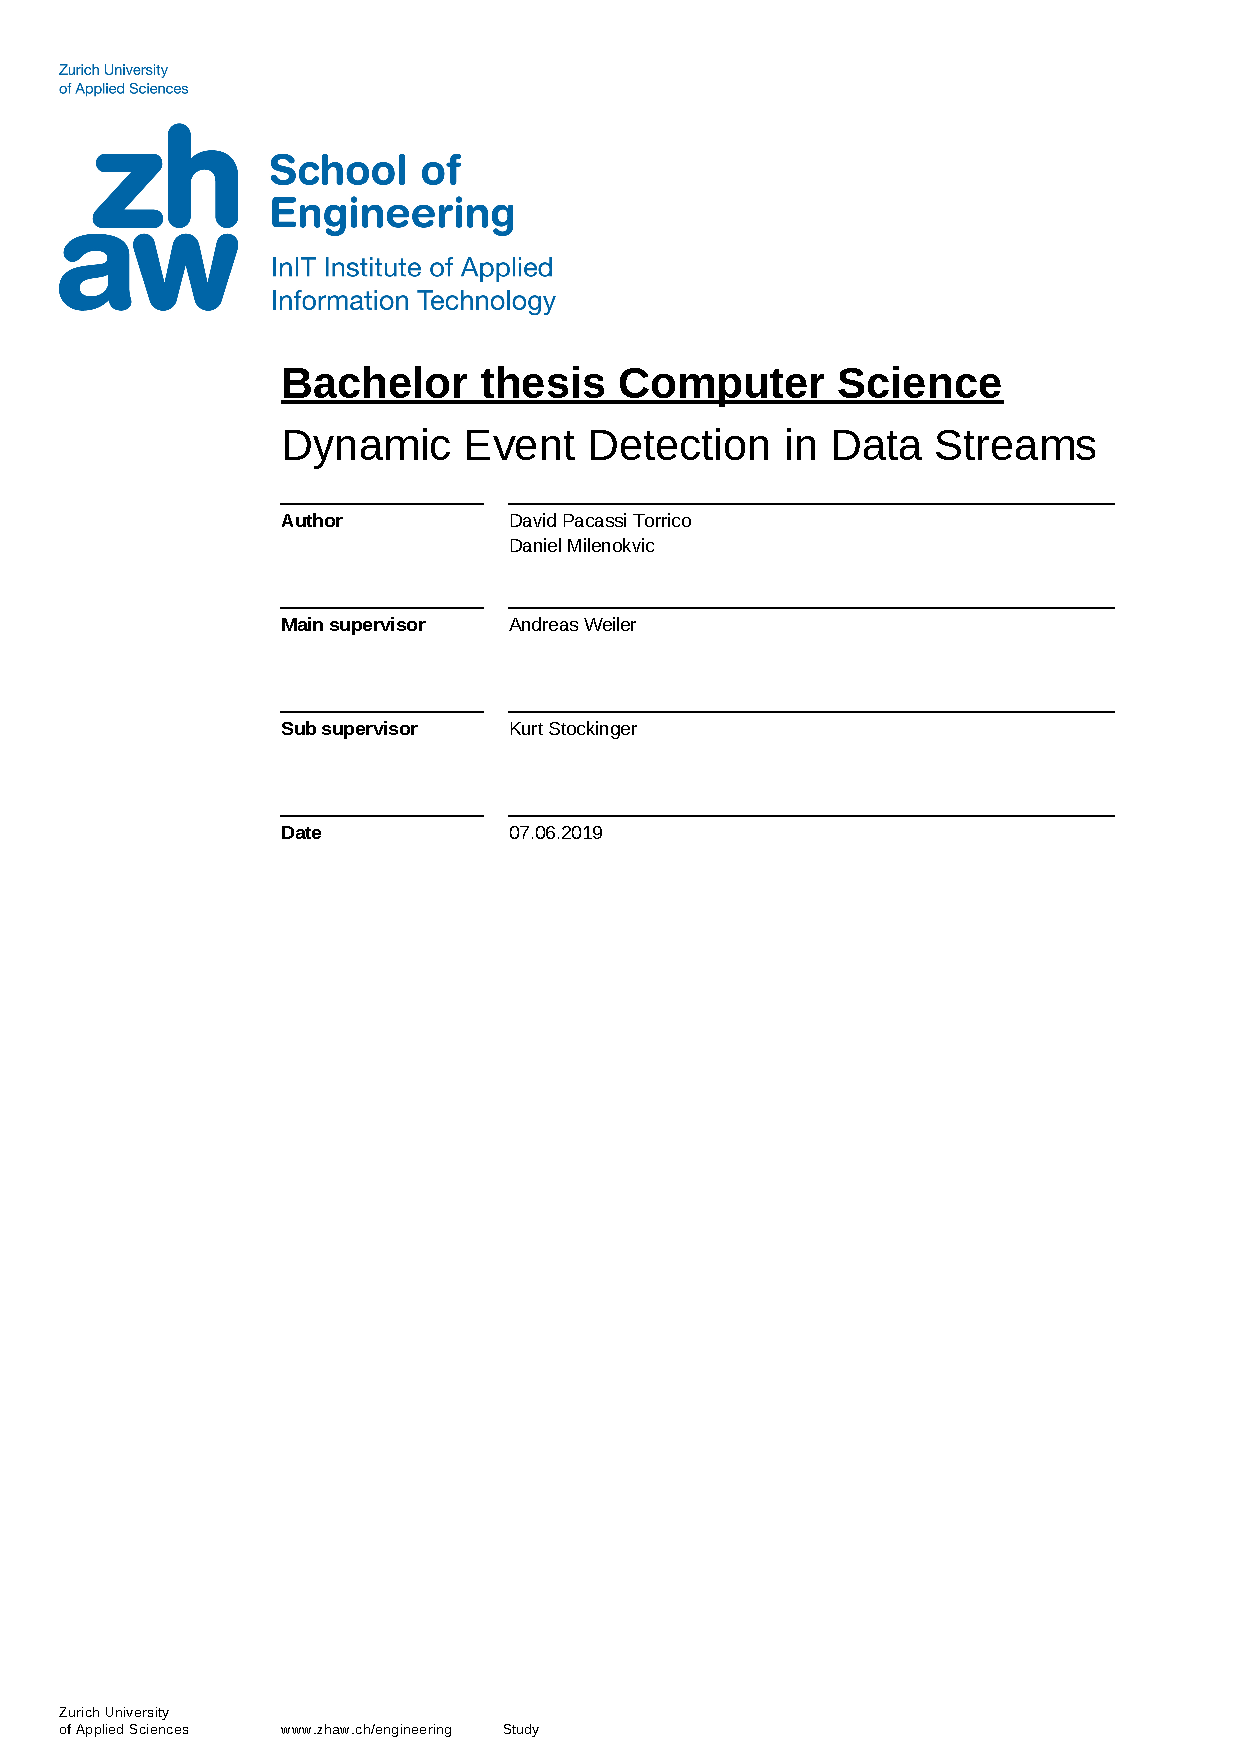
\includepdf{templates/cover.pdf}

\includepdf{templates/declaration_of_originality.pdf}

\tableofcontents\newpage
% Der Umfang des Abstracts sollte nicht mehr als eine A4-Seite sein
% (nach DIN / ISO / ANSI beschränkt sich ein Abstract auf ca. 250 Wörter, also eine halbe A4-Seite).

\section{Abstract}

% Einleitung: definiert die Problematik und begründet die Relevanz der Arbeit.
How can events be recognized in a data streams?
And what is the definition of an event?
Current event recognition procedures define possible events (or event types) statically when the system starts.
However, in data streams, the definition should develop dynamically over time as the data and their focus changes over time.

% Methodische Einordnung der Arbeit: Art, Datenbasis und Ziel der Arbeit.
The first goal of this bachelor thesis is to define what an event is and how events can be recognized from static data.
Depending on the definition, a suitable dataset has to be found and chosen in order to create a system
which is capable of recognizing events.
In the second part, the events should be recognized from a data stream and therefor support dynamic event recognition.

% Vorgehen: informiert exemplarisch über die Untersuchungsanlage.
This work uses news API's as data streams and tries to assign the received news articles to different events.
An event is defined as a list of different news articles writing about the same story.
A possible event could be "Brexit" or an upcoming election.
It's important to keep in mind that new events can and should be created over time.

% Ergebnis: beschreibt die wichtigsten Resultate, Erkenntnisse, offenen Fragen.
Assigning news articles to an event can be done by clustering the news articles.
In order to achieve best possible results, a comparison between different clustering techniques has been completed.
It was revealed that HDBSCAN is a promising candidate for our use case as it delivered the best results.

Unfortunately HDBSCAN was not made for data coming from data streams but this thesis will show
one possible solution on how to deal with this.
This work as able to process up to 20'000 news articles with HDBSCAN.
A possible continuation of this work could try to extend this number to process more data at once.

\section{Einführung}

Wie kann in einem Datenstrom Ereignisse erkannt werden?


Bei der Suche nach neuen Ereignissen in Datenströmen, kommt es immer zum Problem was ein Ereignis genau ist. Wenn diese erste Frage geklärt ist kommt es aber zu weiteren Fragestellungen. Meistens reicht es nicht ein Ereignis statisch zu definieren, sondern die Definition entwickelt sich dynamisch über die Zeit. Die meisten Verfahren zu Ereigniserkennung werden aber bei Systemstart statisch eingestellt. Weiterhin muss man stets die Dynamik des Streams beachten, da es sonst du Blockaden und Überlauf im System kommen kann.

Ziel dieser Arbeit ist es eine Methodik zu entwickeln wie die genannten Aspekte auf geeigneten Datenströmen umgesetzt werden können.


\section{Method}

TODO introductionary paragraph

\subsection{Test Data}

The first important step is to create a test data set to run the evaluations with and verify them.

TODO explain the source and structrue

\subsection{Clustering methods}

Clustering finds similarities in different news articles based on their content and groups them together, while unrelated news are regarded as noise. The challenge now araises to find an appropriate clustering method, which is able to work with data of varying densities and of high dimensionality.

TODO why hdbscan

\subsubsection{HDBSCAN}

HDBSCAN is a hierarchical density-based clustering algorithm \cite{McInnes2017}. It extends the well known [insert citation] DBSCAN algorithm and reduces its sensitivity for clusters of varying densities. Another important quality of HDBSCAN is, that it does not need to know the number of clusters up front.

 TODO explain some more

\subsubsection{K-means}

KMeans is a centroid-based clustering algorithm. 

 TODO explain some more

\subsubsection{Preprocessing}

% raw text
% with entity extraction
% word embeddings?
% Tfidf

\subsubsection{Score calculation}

The scoring function is essential for measuring the result of a clustering method. The score should tell us how close the resulting clusters are to the ground truth and give us an intuitive understanding about the quality of the clusters. One of the challenges when comparing one clustering with the other, is that the differnet clusters do not share the same label across different clusterings. Which is why scoring functions used for clusterings typically ignore the labels and focus on the shape of a cluster.

Initially we used Normalized Mutual Information (NMI) as our primary scoring function. The NMI calculates the mutual information between two clusterings and normalizes the result by dividing through a generalized mean of the entropy of each clustering. % TODO better description.
The score proved to work well for our initial evaluations and manual samplings verified the score. Upon running evaluations with higher sample sizes the NMI score started to lose its reliability. An example is given in Table \ref{tab:nmi_kmeans_example}, where K-means achieved a rather high score, regardless to the significant difference between the true amount of clusters and the approximation using $\sqrt{n}$.

% TODO explain the reason for the big difference

TODO add number of estimated clusters
\begin{table}[h]
    \centering
    \begin{tabular}{|l|l|l|l|}
    \hline
    \textbf{Algorithm} & \textbf{Sample Size} & \textbf{NMI}  & $\mathbf{ \mid n_{true} - n_{predicted} \mid }$ \\ \hline
    k-means & 19255 & 0.754 & 457 \\ \hline
    hdbscan & 19255 & 0.742 & 2 \\ \hline
    \end{tabular}
    \caption{K-Means has a higher NMI score than HDBSCAN, while having a much larger difference in number of clusters.}
    \label{tab:nmi_kmeans_example}
\end{table}

To get a more accurate score based on the documents inside a cluster, we developed our own scoring function. 

\paragraph{Calculating the score}

The scoring function first calculates the accuracy for each combination of two clusters, where each clusters belongs to a different clustering. We define the accuracy as

\begin{equation}
    \label{equ:accuracy}
    \frac{n_{true}}{n_{true} + fp + fn}
\end{equation}

where $n_{true}$ is the number of elements in the true cluster, $fp$ is the number of false positives in the predicted cluster and $fn$ describes the number of false negatives in the predicted cluster. To illustrate this step with an example, we use $T$ and $C$ as our clusterings, where $T$ is the true clustering and $C$ is the predicted clustering. The clusterings are defined as follows:

\begin{gather*}
    T = \{\{1,2,3\},\{4,5,6,7\},\{8,9\}\} \\
    C = \{\{1,2\},\{3,4,5,6\},\{7\},\{8,9\}\}
\end{gather*}

We calculate the accuracy as defined in Equation \ref{equ:accuracy}, for each possible pair between $T$ and $C$ starting with $t_1= \{1,2,3\}$ and $c_1 = \{1,2\}$:

\begin{align*}
    accuracy(t_1,c_1) &= \frac{n_{true}}{n_{true} + fp + fn} \\
    &= \frac{|t_1|}{|t_1| + |c_1 - t_1| + |t_1 - c_1|} \\
    &= \frac{3}{ 3 + |\{\emptyset\}| + |\{3\}|} = \frac{3}{ 3 + 0 + 1} \\
    &= \frac{3}{4} = 0.75 \\
\end{align*}

After doing this for each possible pair we get the accuracy matrix $A$:

\begin{gather*}
\begin{array}{rcl}
    A = & \left(\begin{array}{cccc}
        accuracy(t_1,c_1) & \hdots & \hdots & accuracy(t_1,c_4)\\
        \vdots & \vdots & \vdots & \vdots\\
        accuracy(t_3,c_3) & \hdots & \hdots & accuracy(t_3,c_4) \end{array}\right)
        = & \left(\begin{array}{cccc}
            0.75 & 0.375 & 0.427 & 0.375 \\
            0.4 & 0.667 & 0.571 & 0.4 \\
            0.333 &  0.25 & 0.4 & 1.0 \end{array}\right)
\end{array}
\end{gather*}

As a next step we have to select the most relevant accuracy values from each row of the accuracy matrix. 

Finding relevant values in the accuracy matrix non-trivial, since clusters do not share labels across different clusterings. To solve this, we make two assumptions:
\begin{enumerate} 
\item The higher the accuracy between two clusters, the more likely it is, that both clusters are describing the same group of documents. 
\item Each cluster can be associated with a cluster from another clustering only once.
\end{enumerate}

Based on those assumptions we select the highest accuracy value per row, whose column is not already associated with another row. Applying this selection function $f$ to our previously calculated accuracy matrix $A$ results in the set containing the most relevant accuracy values.

\begin{gather*}
    \begin{array}{rcl}
        f(A) = & \left(\begin{array}{cccc}
                \mathbf{0.75} & 0.375 & 0.427 & 0.375 \\
                0.4 & \mathbf{0.667} & 0.571 & 0.4 \\
                0.333 &  0.25 & 0.4 & \mathbf{1.0} \end{array}\right)
            = \{0.75, 0.667, 1\}
    \end{array}
\end{gather*}

As we can see, there were no collisions between columns and we simply get the highest value per row. Consider the following example with an accuracy matrix $B$, which does contain a collision:

\begin{gather*}
    \begin{array}{rcl}
        f(B) = & \left(\begin{array}{cccc}
            \mathbf{0.75} & 0.375 & 0.427 & 0.375 \\
            0.4 & \mathbf{0.667} & 0.571 & \textcolor{red}{0.8} \\
            0.333 &  0.25 & 0.4 & \mathbf{1.0} \end{array}\right)
            = \{0.75, 0.667, 1\}
    \end{array}
\end{gather*}

The selected accuracy for the second row is 0.667 instead of 0.8. This is because the fourth column is already associated with the third row, while having an accuracy greater than 0.8. Therefore based on our assumption that clusters cannot be associated twice, the second highest accuracy is used for the second column. In case no association could be found, the value would be set to zero. The full algorithm for the selection process can be found in the appendix as listing \ref{lst:select_max_values}.

As a final step the average is calculated from the sum of the accuracy with respect to the difference in predicted clusters to the true amount of clusters. In case the predicted amount is lower a normal average will already result in a lower score, since each real cluster without a matching predicted cluster counts as zero. However if there are more predicted clusters than true ones, each true cluster will have a value and the score would appear the same as if there was a perfect prediction in the amount of clusters. To take this into account, the difference is added to the number of true clusters as shown in Equation \ref{equ:avg_accuracy}.

\begin{equation}
    \label{equ:avg_accuracy}
        \frac{s_{accuracy}}{c_{true} + max(0, c_{predicted} - c_{true})}
\end{equation}

Where $s_{accuracy}$ is the sum of the accuracy values, $c_{predicted}$ is the number of predicted clusters and $c_{true}$ is the number of true clusters. Using our previously selected accuracy values $S = f(A) = \{0.75, 0.667, 1\}$ with  $c_{true}=3$ and $c_{predicted}=4$, the calculation for the final average would be done as follows:

\begin{align*}
    score &= \frac{\sum_{i=1}^{|S|} S_i}{c_{true} + max(0, c_{predicted} - c_{true})} \\
    &= \frac{0.75 + 0.667 + 1}{3 + max(0, 4 - 3)} = \frac{2.417}{3 + max(0, 1)} \\
    &= \frac{2.417}{3 + 1} = \frac{2.417}{4} \\
    &= \mathbf{0.604}
\end{align*}

The final score for the evaluation of the predicted cluster $C$ with the true cluster is 0.604.

\paragraph{Comparison against NMI}

After repeating the evaluation shown in Table \ref{tab:nmi_kmeans_example} a second time using the average accuracy per clustering, the score (Table \ref{tab:avg_predict_kmeans_example}) for K-means is much lower than HDBSCAN. This reflects what we would expect based on the big difference in the amount of predicted clusters.

\begin{table}[h]
    \centering
    \begin{tabular}{|l|l|l|l|}
    \hline
    \textbf{Algorithm} & \textbf{Sample Size} & \textbf{Accuracy}  & $\mathbf{ \mid n_{true} - n_{predicted} \mid }$ \\ \hline
    k-means & 19255 & 0.137 & 457 \\ \hline
    hdbscan & 19255 & 0.605 & 2 \\ \hline
    \end{tabular}
    \caption{K-Means has a higher NMI score than HDBSCAN, while having a much larger difference in number of clusters.}
    \label{tab:avg_predict_kmeans_example}
\end{table}

The test scenarios in table \ref{tab:score_scenarios} show the resulting scores of our accuracy score, NMI and completeness. It is important to note that NMI and completeness work with cluster labels assigned to each document, instead of considing elements inside a single cluster. This means the clustering will be flattened into one dimension, where each document is assigned the label of the cluster it appeares in. The array containing the labels for the first scenario would look as follows: $C=[1,1,1,2,2,2,2,3,3]$.

\begin{table}[h]
    \centering
    \begin{tabular}{|l|l|l|l|l|}
    \hline
    \multicolumn{5}{ |c| }{\textbf{Test scenarios with true clustering $T = \{\{1,2,3\},\{4,5,6,7\},\{8,9\}\}$}} \\
    \hline
    Nr. & Predicted Clustering $C$ & NMI & Completeness & Accuracy \\ \hline
    1 & $C = \{\{1,2,3\},\{4,5,6,7\},\{8,9\}\}$ & 1.0 & 1.0 & 1.0 \\ \hline
    2 & $C = \{\{1,2\},\{3,4,5,6\},\{7,8,9\}\}$ & 0.564 & 0.564 & 0.694 \\ \hline
    3 & $C = \{\{1,2,3\},\{4,5,6\},\{7\},\{8,9\}\}$ & 0.895 & 0.809 & 0.7 \\ \hline
    4 & $C = \{\{1,2,3\},\{4,5\},\{6,7\},\{8\},\{9\}\}$ & 0.821 & 0.697 & 0.467 \\ \hline
    5 & $C = \{\{1\},\{2\},\{3\},\{4\},\{5\},\{6\},\{7\},\{8\},\{9\}\}$ & 0.651 & 0.483 & 0.204 \\ \hline
    6 & $C = \{\{1,2,3,4,5\},\{6,7,8,9\}\}$ & 0.434 & 0.552 & 0.367 \\ \hline
    7 & $C = \{\{1,2,3,4,5,6,7,8,9\}\}$ & 0.0 & 1.0 & 0.148 \\ \hline
    8 & $C = \{\{7,2,4\},\{8,9,6,3\},\{1,5\}\}$ & 0.219 & 0.219 & 0.524 \\ \hline
    \end{tabular}
    \caption{Direct comparison of different scoring functions}
    \label{tab:score_scenarios}
\end{table}

TODO explain scores. why is it better than NMI?

\subsection{Online Clustering}

* time based sliding window
* Near duplicate detection for clusters with MinHash and LSH O(log n)
* Jaccard Coefficient: number of common elements / (total number of elements - number of common elements)
* source https://towardsdatascience.com/understanding-locality-sensitive-hashing-49f6d1f6134
* defining events -> new story, changes in story (additions/deletions)

\section{Implementation}
% or implementation?

\subsection{Evaluation Framework}
The evaluation process is done with our own evaluation framework. The framework allows for automated and repeatable evaluation runs. Results are stored in a database for later analysis. The main features include:

\begin{itemize}
    \item Defining the number of stories to run the evaluation with and load all news articles from those stories. 
    \item Repeating evaluation runs with different sets of data.
    \item Providing different vectorizers for converting the textual data into a vector space model.
    \item Defining a range for each parameter of a clustering method and running it with each possible combination of those parameters. 
    \item Storing the result the result in a database and creating relations between news articles, clusters and evaluation runs. This allows for manual inspection and analysis of individual articles inside a predicted cluster. 
\end{itemize}

The implementation is done with Python. Clustering methods and vectorizers are provided by the Scikit-learn library. We decided to use Scikit-learn because of its rich documentation, the wide range of tools and algorithms it provides for clustering and our previous experience with it. Additionally the framework runs in a fully dockerized environment, which includes the database. This makes it very easy to run locally or on a server. 

% TODO write it better

\subsection{Online Clustering}

* Near duplicate detection for clusters with MinHash and LSH O(log n)
* source https://towardsdatascience.com/understanding-locality-sensitive-hashing-49f6d1f6134

* simulate an dynamic stream from our static dataset
\section{Results}

\subsection{Clustering method}

The goal of this evaluation is to measure the accuracy of HDBSCAN, with different parameters and preprocessing methods. The most suitable approach will then be used for the online clustering to detect changes in a news stream.

\subsubsection{Setup}

\paragraph{Text Preprocessing}

 The first step in working with text is to apply Natural Language Processing techniques for improving the quality of the data before clustering it. We look the five different preprocessing methods  as described in section \ref{} and evaluate each. The methods are:
 \begin{itemize}
     \item Full text with stop word removal
     \item Keyterms
     \item Named Entities
     \item Lemmatization
     \item Stemmatization
 \end{itemize} 

\paragraph{Text Vectorization} Before the text can be clustered, it has to be transformed into a vector space model. We look at two different models:
\begin{itemize}
    \item Word Count
    \item Tfidf
\end{itemize}

\paragraph{Parameters} HDBSCAN has a range of parameters, which can be tuned to fit our dataset. We focus on the two primary ones:
\begin{itemize}
    \item Min cluster size: The minimum size of a cluster. We run the evaluation with a range from two to nine as the $min\_cluster\_size$. 
    \item Metric: The distance measure between points. We apply the metrics "cosine" and "euclidean". 
    
\end{itemize}

The primary parameter for K-Means is the number of clusters. Since K-Means is used as a baseline to evaluate HDBSCAN, we provide the true number of clusters for each run. Therefore K-Means runs with an optimal starting point. 

\paragraph{Running the evaluation} The evaluation is done with different sets of news articles per run. This means if we define a run to use 30 stories and set it to repeat five times, each repeat will load 30 different stories from the dataset. This is done to get a more diverse set of samples. Each run will be repeated at least three times. Lower numbers of stories allow for more repetitions due to lower processing times.   

\subsubsection{Evaluation}

The first run is done with 60 stories, which results in approximately 2000 news articles, over five repetitions. Table \ref{tab:cluster_parameters} shows the resulting accuracy for each parameter in combination with each preprocessing method and vector space model. The highest score per parameter is highlighted as bold. The first insight we get is the variety in accuracy scores for different min cluster sizes. The lowest min cluster size results in the lowest accuracy, while increasing this parameter leads to an increasingly better score. The highest accuracy is reached with a min cluster size of six, while increasing it further reduces the score again. The large difference in accuracies between different min cluster sizes, shows the importance this parameters has on the quality of the clustering and requires some knowledge of the data beforehand. In our case we have a wide range of different cluster sizes as shown in figure \ref{fig:articles_per_story_distribution}, with clusters containing as little as two news articles. Based on this distribution we expected the min size cluster size to be low. The distribution also explains the drop in accuracy after a min cluster size of 6, since an increasingly number of clusters are being ignored.

\begin{table}[h]
    \centering
    \scalebox{0.65}{
    \begin{tabular}{|l|rrrrr|rrrrr|}
        \hline
        \textbf{Clustering} & \multicolumn{5}{ |c| }{\textbf{Word Count}} & \multicolumn{5}{ |c| }{\textbf{Tfidf}} \\
        \hline
        \textbf{HDBSCAN} & Full Text &  Keyterms & Entities & Lemmatized & Stemmed & Full Text &  Keyterms & Entities & Lemmatized & Stemmed \\
        \hline
        min\_size: 2, metric: cosine    & 0.289 & 0.265 & 0.223 & \textbf{0.305} & 0.297 & 0.286     & 0.268 & 0.26      & 0.296     & 0.3       \\
        min\_size: 2, metric: euclidean & 0.101 & 0.093 & 0.110 & 0.101     & 0.106 & 0.301     & 0.170 & 0.241     & \textbf{0.306} & 0.301     \\
        min\_size: 3, metric: cosine    & 0.488 & 0.456 & 0.465 & 0.48      & 0.487 & 0.472     & 0.446 & 0.457     & \textbf{0.493} & 0.478     \\
        min\_size: 3, metric: euclidean & 0.172 & 0.129 & 0.176 & 0.174     & 0.182 & 0.472     & 0.306 & 0.464     & \textbf{0.500} & 0.478     \\
        min\_size: 4, metric: cosine    & 0.630 & 0.555 & 0.625 & 0.552     & 0.577 & 0.577     & 0.586 & \textbf{0.646} & 0.589     & 0.581     \\
        min\_size: 4, metric: euclidean & 0.320 & 0.182 & 0.214 & 0.315     & 0.332 & 0.611     & 0.416 & 0.559     & 0.613     & \textbf{0.615} \\
        min\_size: 5, metric: cosine    & 0.716 & 0.652 & 0.656 & \textbf{0.718} & 0.718 & 0.688     & 0.664 & 0.632     & 0.686     & 0.692     \\
        min\_size: 5, metric: euclidean & 0.355 & 0.217 & 0.266 & 0.41      & 0.389 & \textbf{0.703} & 0.512 & 0.607     & 0.686     & 0.692     \\
        min\_size: 6, metric: cosine    & 0.693 & 0.715 & 0.608 & 0.701     & 0.708 & 0.738     & 0.729 & 0.613     & \textbf{0.751} & 0.747     \\
        min\_size: 6, metric: euclidean & 0.179 & 0.280 & 0.292 & 0.202     & 0.164 & 0.738     & 0.408 & 0.622     & \textbf{0.778} & 0.763     \\
        min\_size: 7, metric: cosine    & 0.631 & 0.611 & 0.552 & 0.643     & 0.634 & 0.689     & 0.685 & 0.553     & 0.718     & \textbf{0.722} \\
        min\_size: 7, metric: euclidean & 0.122 & 0.392 & 0.307 & 0.073     & 0.099 & 0.689     & 0.336 & 0.539     & 0.718     & \textbf{0.722} \\
        min\_size: 8, metric: cosine    & 0.571 & 0.603 & 0.514 & 0.592     & 0.574 & 0.685     & 0.647 & 0.531     & \textbf{0.711} & 0.695     \\
        min\_size: 8, metric: euclidean & 0.056 & 0.339 & 0.338 & 0.025     & 0.057 & 0.685     & 0.286 & 0.522     & \textbf{0.711} & 0.695     \\
        min\_size: 9, metric: cosine    & 0.542 & 0.569 & 0.476 & 0.544     & 0.541 & 0.602     & 0.614 & 0.499     & 0.637     & \textbf{0.640} \\
        min\_size: 9, metric: euclidean & 0.065 & 0.236 & 0.310 & 0.025     & 0.033 & 0.602     & 0.216 & 0.475     & 0.637     & \textbf{0.640} \\
        \hline
        \textbf{K-Means} & \multicolumn{5}{ |c| }{}  & \multicolumn{5}{ |c| }{} \\
        \hline
        n\_cluster: n\_true              & 0.531 & 0.588 & 0.514 & 0.536     & 0.536 & \textbf{0.713} & 0.653 & 0.584     & 0.672     & 0.693     \\
        \hline
    
    \end{tabular}   
    }
    \caption{Accuracy for combinations of parameter and preprocessing with a sample size of 60 stories (approx. 2000 articles)}
    \label{tab:cluster_parameters}
\end{table}

Comparing the two vector models, shows the majority of best scores per parameter achieved by Tfidf. Additionally the different metrics show a significant difference when using the vector model based on word count. With Tfidf the difference between both metrics is often negligible.

As for the optimal preprocessing, lemmatization appears to provide the highest accuray in general or at least being fairly close to the highest score. This is to be expected, since lemmatization reduces the dimensions by grouping words into their base form, while still retaining most of the text. In contrast to keyterm and entity extraction, which both result in a drastic reduction of the dimensions, and therefore less detail. It is important to note, that we used pretrained models for keyterm and entity extraction. Specifically training on a news corpus might improve the performance of both methods, but it was decided as to be out of scope for this thesis.

\begin{figure}[h]
    \centering
    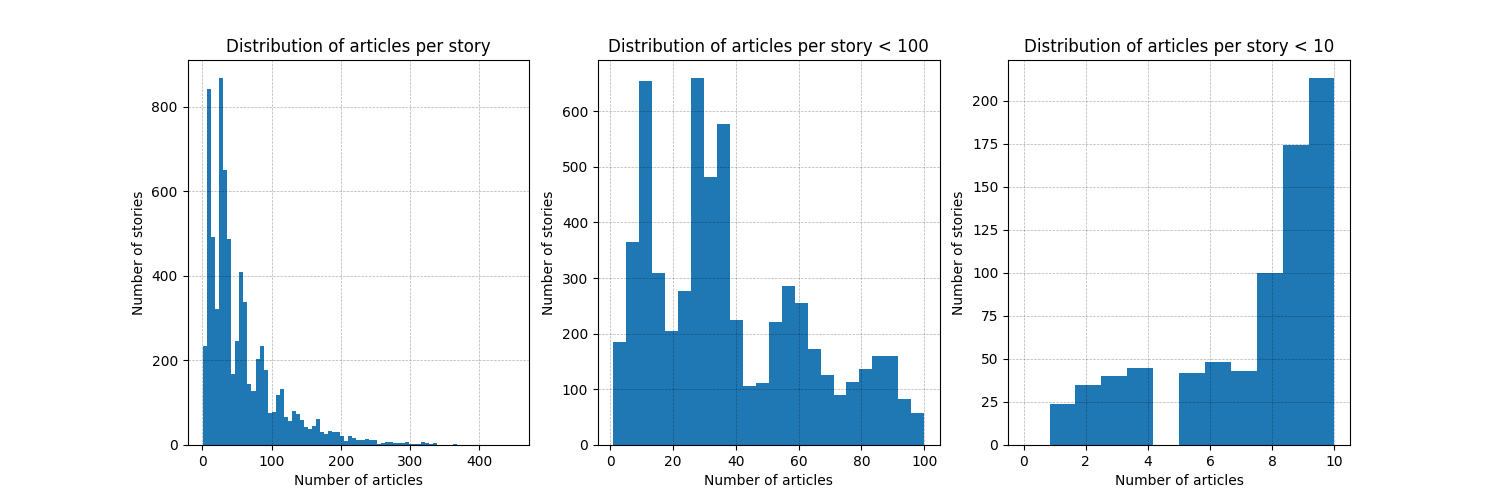
\includegraphics[width=1\textwidth]{articles_per_story_distribution}
    \caption{Distribution of cluster sizes.}
    \label{fig:articles_per_story_distribution}
\end{figure}

After determining the optimal settings for text preprocessing and vectorization, we increase the sample sizes for our evaluation runs, to get a deeper insight into the behaviour of HDBSCAN with larger datasets. Figure \ref{fig:hdbscan_parameters} shows the scores achieved with different parameters over an increasingly large set of samples. Based on this figure we see the metric $cosine$ to be generally better than $euclidean$, even if $euclidean$ is occasionally more accurate.

TODO explain why cosine is generally better than euclidean
TODO explain min cluster sizes, but run with lemmatization

\begin{figure}[h]
    \centering
    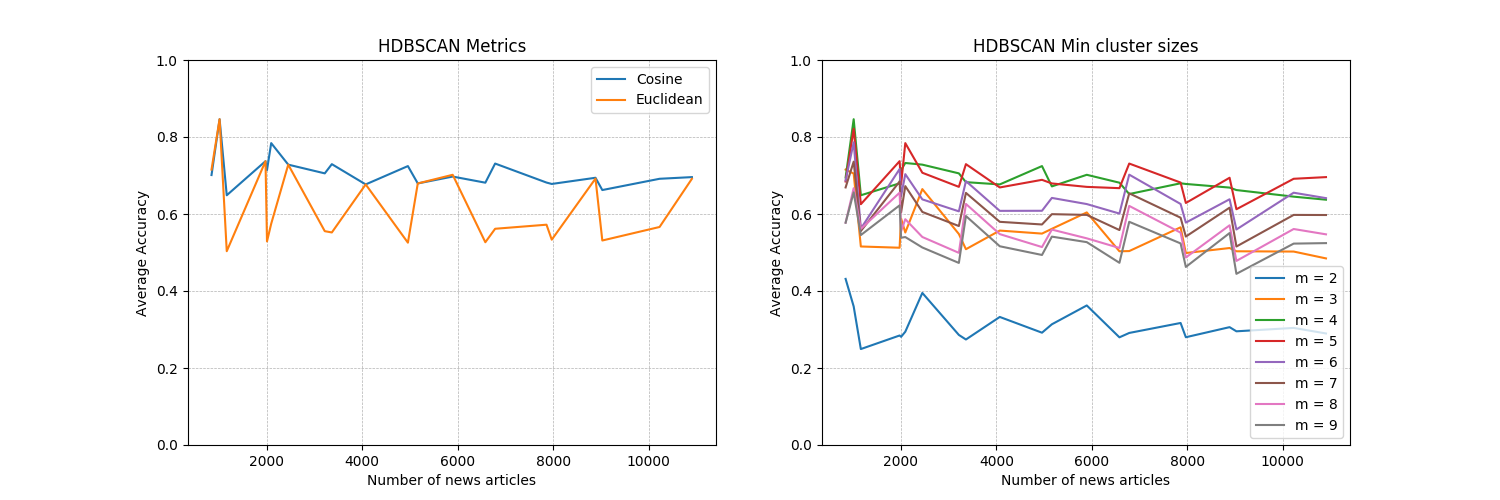
\includegraphics[width=1\textwidth]{hdbscan_parameters}
    \caption{Accuracies for different parameters}
    \label{fig:hdbscan_parameters}
\end{figure}

One of the advantages HDBSCAN has over other clustering algorithms, is the ability to work with noise, since we intent on applying it in an online setting, where noisy data is to be expected. At the same time, the number of articles classified as noise should be kept to a minimum. However the noise ratio shown in Figure \ref{fig:noise_ratio_samples} is higher, than we would expect it to be based on our test data. A variety of factors play into the high noise ratio. One major influence is due to the used $min\_cluster\_size$. Each news article belonging to a cluster ignored due to a size too small, will be counted as noise. In addition to the false positives due to the min cluster size, the test data does still contain noisy data, even after our efforts in cleaning up the data as good as possible. Nontheless the expected noise ratio based on the test data is less than 10\%, nowhere close to the 20\% of the current evaluation. Decreasing the noise ratio is certainly an important part in future improvements.

TODO calculate expected noise ratio based our min cluster sizes.

% experiment with min_samples

\begin{figure}[h]
    \centering
    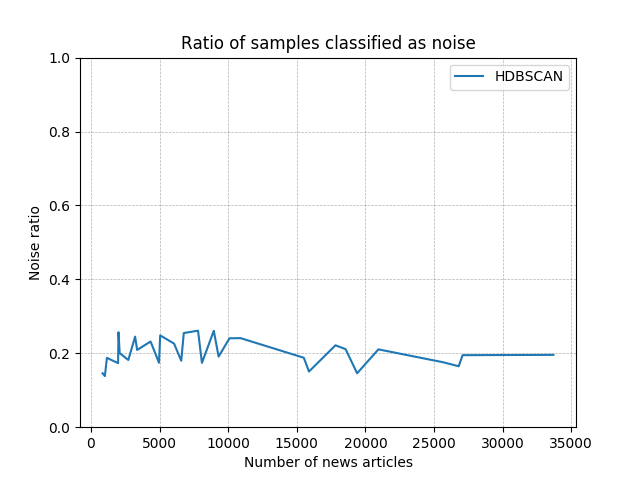
\includegraphics[width=0.5\textwidth]{noise_ratio_samples}
    \caption{Number of news articles classified as noise.}
    \label{fig:noise_ratio_samples}
\end{figure}


Having found the optimal settings to run HDBSCAN with, we can start comparing the overall performance with K-Means. Figure \ref{fig:accuracy_kmeans_hdbscan} shows  a similar behaviour for both clustering methods in value and variance of the accuracy. Although HDBSCAN is generally more accurate than K-Means, the difference gets smaller with an increase in the sample size. 

Increasing the sample size results for both HDBSCAN and K-means in a small loss regarding the accuracy as can be seen in figure \ref{fig:accuracy_kmeans_hdbscan}. However the accuracy seems to stabilize around the 0.7 mark.

\begin{figure}[h]
    \centering
    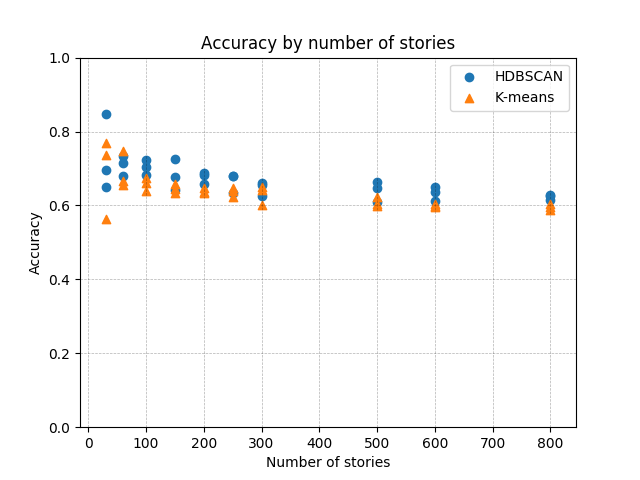
\includegraphics[width=0.5\textwidth]{accuracy_kmeans_hdbscan}
    \caption{Comparison of the average accuracy between K-means and HDBSCAN}
    \label{fig:accuracy_kmeans_hdbscan}
\end{figure}

While HDBSCAN and K-means provide a similar accuracy, the biggest difference can be noted in the processing time in relation to the number of samples. K-means has a time complexity of $O(n^2)$ in contrast to HDBSCAN with a time complexity of $O(nlog(n))$, which is demonstrated by figure \ref{fig:processing_time_kmeans_hdbscan}. Although running the evaluation has also shown the space complexity for HDBSCAN to be substantially higher for larger amounts of samples than with K-means. Trying to run HDBSCAN with 100'000 news articles caused in a memory error, even with 64GB of RAM, while K-means was able to complete the clustering.

% TODO measure memory?

\begin{figure}[h]
    \centering
    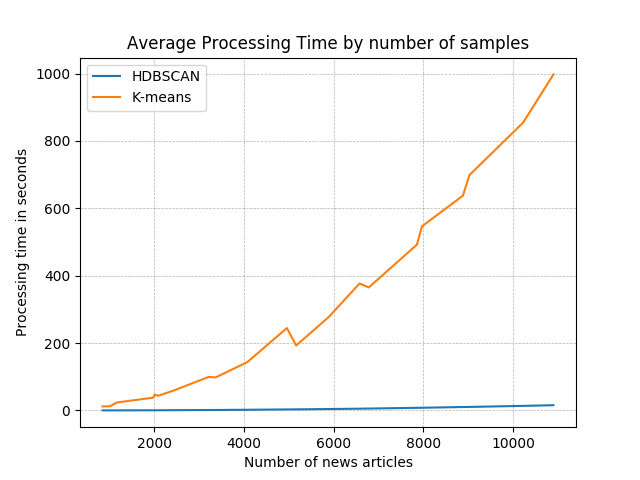
\includegraphics[width=0.5\textwidth]{processing_time_kmeans_hdbscan}
    \caption{Processing time in seconds }
    \label{fig:processing_time_kmeans_hdbscan}
\end{figure}

Figure \ref{fig:cluster_difference_samples} shows, that the difference between predicted over the true number of clusters is fairly low and appears to be roughly linear with the overall number of clusters.  

\begin{figure}[h]
    \centering
    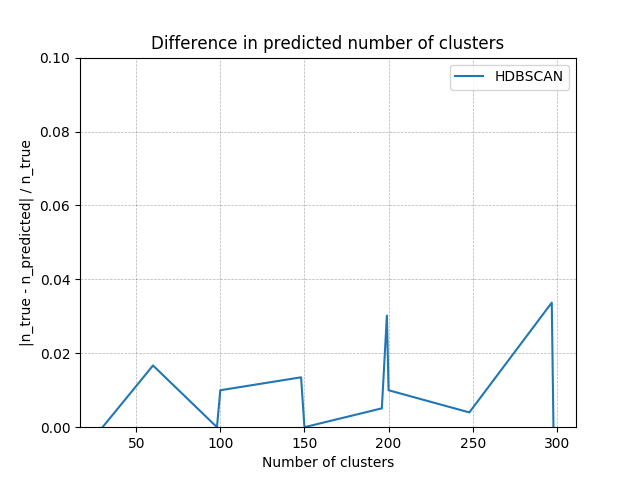
\includegraphics[width=0.5\textwidth]{cluster_difference_samples}
    \caption{Ratio of difference over predicted with true number of clusters}
    \label{fig:cluster_difference_samples}
\end{figure}

As a final note, we compare HDBSCAN with six different clustering methods taken from scikit-learn. Each method is run with a variety of parameters and the best scores are shown in figure \ref{fig:different_clusterings}. HDBSCAN provides the highest accuracy, while being still being one of the fastest algorithms. Based on this data, we can assume HDBSCAN to be a good candidate for our use case.

\begin{figure}[h]
    \centering
    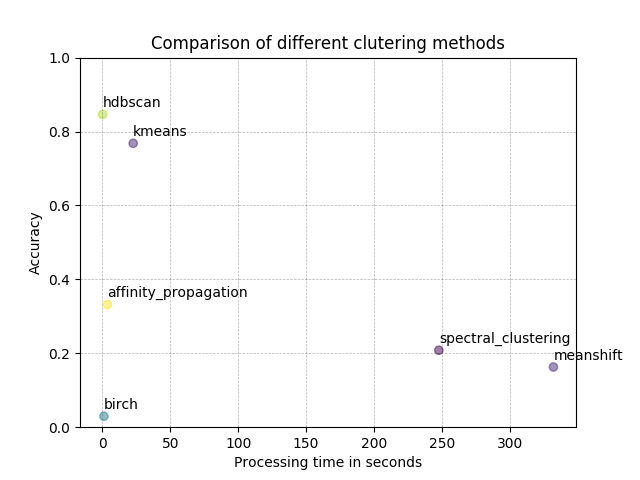
\includegraphics[width=0.5\textwidth]{different_clusterings}
    \caption{Comparison of different clustering methods with a sample size of approximately 1000 news articles}
    \label{fig:different_clusterings}
\end{figure}

\subsubsection{Conclusion}

The evaluation has shown HDBSCAN to be a good candidate to use for news clustering. It provides an better accuracy than K-means, while being significantly faster to process. The predicted number of clusters is consistent with an increasing number of samples and fairly close the truth. Additionally we have shown the required preprocessing and vectorization steps with the ideal parameters to achieve the most accurate results for our dataset. On the flip side the noise ratio is quite high and the space complexity is problematic with larger datasets. Overall HDBSCAN provides an acceptable accuracy, while still leaving room for further improvements.

\subsection{Evaluation of online clustering}

TODO new topic, topic extended

TODO cluster stability

\begin{figure}[h]
    \centering
    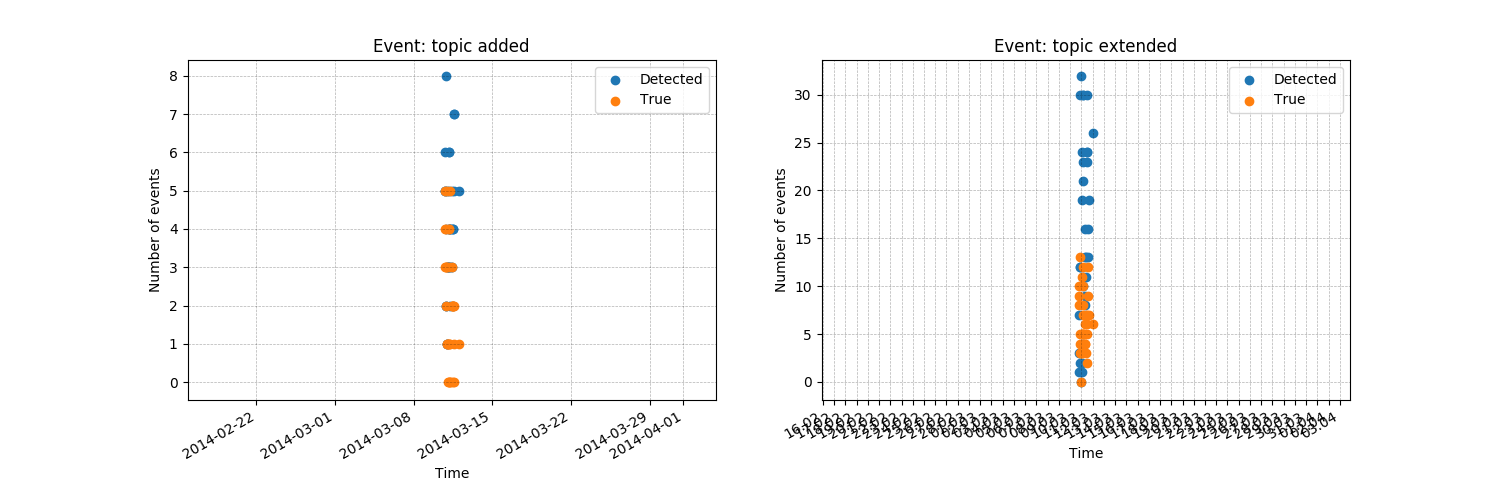
\includegraphics[width=1\textwidth]{event_detection_by_date}
    \caption{Comparison between detected and true events}
    \label{fig:event_detection_by_date}
\end{figure}

\begin{figure}[h]
    \centering
    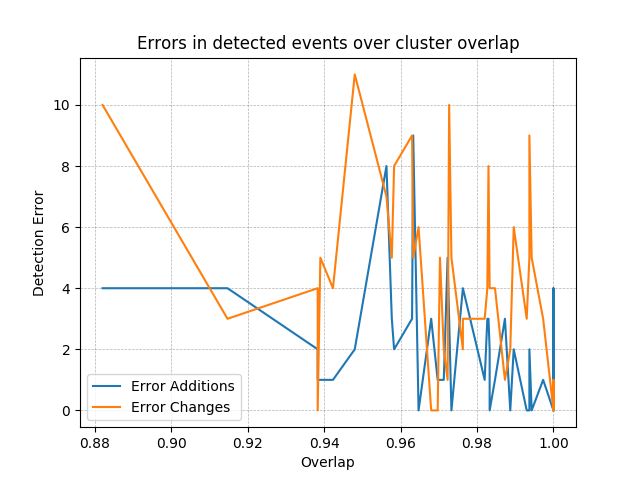
\includegraphics[width=0.5\textwidth]{event_detection_overlap}
    \caption{Plot work in progress}
    \label{fig:event_detection_overlap}
\end{figure}

% analyse overlap size
% show incoming news articles
% show deletion events on full clusterings
\section{Conclusion}

\subsection{Summary}

Short summary of this work.

\subsection{Advantages and Drawbacks}

What are the Advantages and Drawbacks of our work?

\subsection{Further Improvements}

How can this work be improved further? % Diskussion und Ausblick
\section{Appendix}

\subsection{Algorithm for Accuracy Selection}

\begin{lstlisting}[language=Python, caption=Select relevant accuracy values from a accuracy matrix., label={lst:select_max_values}]
    def select_max_values(self, accuracy_matrix):
        unique_indicies = dict()
        row_index = 0
        nrows = len(accuracy_matrix)
        
        while row_index < nrows:
            ignore_indicies = set()
            max_value_found = False
    
            while not max_value_found:
                max_value = 0
                column = 0
                for col_index, value in enumerate(accuracy_matrix[row_index]):
                    if value >= max_value and col_index not in ignore_indicies:
                        max_value = value
                        column = col_index
    
                if (
                    max_value > 0
                    and column in unique_indicies
                    and unique_indicies[column]["row_index"] != row_index
                    and unique_indicies[column]["max_value"] > 0
                ):
                    if unique_indicies[column]["max_value"] < max_value:
                        # The column is already used, but we found a better 
                        # candidate. We use the new candidate and set the 
                        # cursor to the old one to find a new max value.
                        old_row_index = unique_indicies[column]["row_index"]
                        unique_indicies[column]["row_index"] = row_index
                        row_index = old_row_index
                        unique_indicies[column]["max_value"] = max_value
                        max_value_found = True
                    else:
                        # The column is already used by a better candidate.
                        ignore_indicies.add(column)
                else:
                    # If max_value is greater than 0, we store the value as a 
                    # new candiate. Otherwise either the row does not match 
                    # any other column or the max_value was low and got 
                    # overriden by previous tries and no other match is available. 
                    if max_value > 0:
                        # The column is free to use
                        unique_indicies[column] = {
                            "row_index": row_index,
                            "max_value": max_value,
                        }
                    max_value_found = True
                    row_index += 1
        
        return unique_indicies
\end{lstlisting}
    


% \bibliography{citations}

\end{document}

